\documentclass{article}
\usepackage{graphicx}
\usepackage{amsmath}
\begin{document}
Tameez Latib

Problem 16

I, Tameez Latib, declare that this work is my own. I did this work honestly and can fully stand behind everything that I have written.

----

Given \$1000, and three stock choices, A, B, and C (described below) how should we invest?


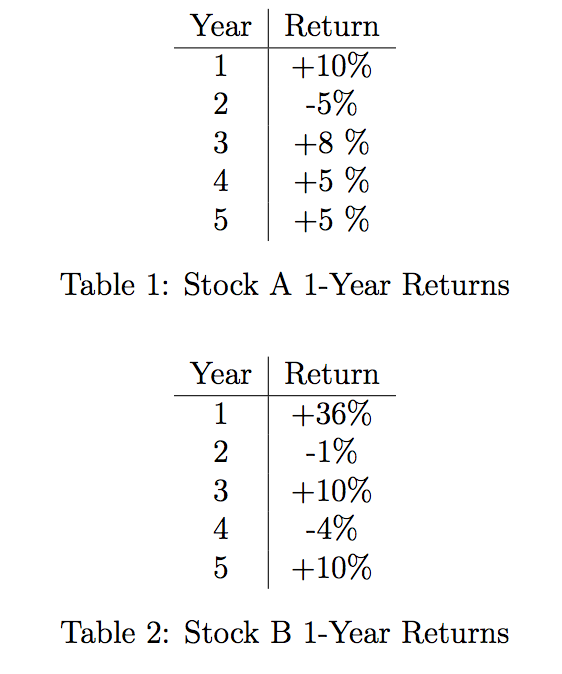
\includegraphics[width=8cm, height=10cm]{StockAB}

\vspace{1cm}

Stock C: guaranteed 3\% return.

Let's assume that each return is equally likely. Now we can find the expected value for stocks A and B. 

For A:

$$E_A = \frac{10 - 5 + 8 + 5 + 5}{5} \% = 5.6\%$$

For B:

$$E_B = \frac{36 - 1 + 10 - 4 + 10}{5} \% = 10.2\%$$

Simply from the analysis of the expected returns, it seems that stock B is the best, with A coming in second. However, we should also take into account the risk. For stock C, there is no risk, but we are left with the smallest return. For Stock A, there is a 20\% chance of losing money, and for stock B, there is a 40\% chance of losing money. However, these losses are almost negligible; ~\$50 or less (less than 5\% of \$1000). Furthermore, stock B has a 20\% chance to gain a large amount of money, ~\$360. For this reason, I would \textbf{invest all of it in stock B}, as it is the only stock worth investing in. Losing money in stock B is negligible, but gaining money actually means something. For stock C, gaining ~\$30 over one year is meaningless. Stock A is a less risky option, but provides lower returns.  

\end{document}
